% ============================================================================
\section{Experiments}

\subsection{GroundBench: Multi-Shot Consistency Benchmark}

Recent multi-shot benchmarks have begun to evaluate long-range coherence and story-level consistency, but most remain holistic: they do not localize failures to individual recurring entities, nor isolate the challenge dimension that triggered the failure. As a result, they can show that a method is inconsistent, but not whether the error comes from a particular character, object, or location, or from factors such as viewpoint change, occlusion, multi-identity confusion, or scene revisits. We construct \textbf{GroundBench}, a diagnostic benchmark with both properties. GroundBench is \emph{entity-grounded}: metrics are computed on entity level rather than only full frames, allowing failures to be attributed to specific recurring entities---characters, objects, or locations. It is also \emph{modular}: scripts are organized into diagnostic modules that systematically vary one challenge dimension at a time, enabling fine-grained failure analysis.

\paragraph{Benchmark design.}
GroundBench contains \textbf{54 multi-shot scripts} ($\sim$300 shots total) spanning four diagnostic axes: \emph{identity preservation} under scale/lighting/viewpoint/occlusion changes, \emph{multi-identity discrimination} with visually distinct or similar characters, \emph{structural patterns} such as scene revisits, intercut timelines, long sequences, and late character introduction, and \emph{robustness probes} involving style shifts, crowds, and pronoun-heavy coreference. Each axis is further divided into controlled sub-categories with three difficulty levels; the detailed taxonomy is provided in the supplementary material.

\paragraph{Metrics.}
GroundBench reports diagnostic metrics designed for multi-shot consistency.
Our primary entity-level metrics are: \textbf{ARC} (Anchor-Relative Consistency), which measures whether each recurring entity remains consistent with its first valid appearance; \textbf{WCI} (Worst-Case Identity), which measures the lowest similarity between an entity's first valid appearance and any later occurrence; \textbf{XCD} (Cross-Character Discrimination), which measures the separation between same-character and different-character similarities in multi-identity scenes; and \textbf{EAF} (Entity-Attribute Fidelity), which measures whether each detected entity matches its textual appearance description. We also report \textbf{ESC} (Environment/Scene Consistency) to evaluate whether recurring settings remain visually coherent across shots after foreground entities are masked out.
As a shot-level consistency baseline, we report \textbf{CSC} (Cross-Shot Consistency): the mean pairwise cosine similarity of ViCLIP~\cite{wang2023internvid_viclip} video features across all shot pairs, following prior works~\cite{holocine,multishotmaster,storymem}.
All metrics are computed with a method-independent Unified Evaluation Detector (UED).
For video quality assessment, we additionally report aesthetic quality and dynamic degree from VBench~\cite{huang2024vbench_comprehensive}. Formal definitions are provided in the supplementary material.
% ============================================================================
\subsection{Experimental Setup}

We compare against four multi-shot baselines:
\textbf{HoloCine}~\cite{holocine}, \textbf{MultiShotMaster-1.3B}/\textbf{MultiShotMaster-14B}~\cite{multishotmaster} and \textbf{StoryMem}~\cite{storymem}.
For the experiments reported here, GroundShot uses Vidu~\cite{vidu} as the primary video generation backend for both bootstrap T2V shots and reference-conditioned shots (\texttt{viduq3-pro} and \texttt{viduq3-mix}).
To evaluate backend-agnosticism, we additionally report results with Kling~\cite{kling} as an alternative commercial backend and Wan2.1-T2V~\cite{wan2024wan} + Phantom-14B~\cite{phantom} as a fully open-source backend, all under the same agentic framework.
We use 4-second, 16:9, 720p clips with automatic motion amplitude and audio disabled.
Entity parsing uses GPT-4o~\cite{gpt4o}. GPT-4.1~\cite{gpt41} is used for the LLM-based decisions in scheduling, reference retrieval, and shot verification, such as reference-quality estimation, target-shot reference scoring, and VLM critique.
Entity-level grounding uses ReferDINO~\cite{liang2025referdino} to localize foreground entity candidates. Visual-memory admission follows the type-aware quality checks in Section~\ref{sec:visual_memory}, with a minimum candidate quality of 0.4 and a character face-confidence threshold of 0.3; a candidate becomes the canonical reference when its quality score is at least 0.85.

% ============================================================================
\subsection{Comparison}

\begin{table*}[t]
\centering
\footnotesize
\caption{Quantitative comparison on GroundBench. Best in \textbf{bold}, second-best \underline{underlined}. $\uparrow$: higher is better.}
\label{tab:main_results}
\vspace{0.3em}
\setlength{\tabcolsep}{4pt}
\begin{tabular*}{\textwidth}{@{\extracolsep{\fill}}l|ccccc|cc|cc}
\toprule
\multirow{2}{*}{\textbf{Method}} & \multicolumn{5}{c|}{\textbf{Entity-Level}} & \multicolumn{2}{c|}{\textbf{Shot-Level}} & \multicolumn{2}{c}{\textbf{Quality}} \\
\cmidrule(lr){2-6}\cmidrule(lr){7-8}\cmidrule(lr){9-10}
& \textbf{ARC}$\uparrow$ & \textbf{XCD}$\uparrow$ & \textbf{WCI}$\uparrow$ & \textbf{EAF}$\uparrow$ & \textbf{ESC} & \textbf{FaceSim}$\uparrow$ & \textbf{CSC}$\uparrow$ & \textbf{Aesth.}$\uparrow$ & \textbf{Dyn.} \\
\midrule
HoloCine~\cite{holocine}                    & 0.368 & 0.119 & 0.212 & 0.617 & 0.549 & 0.417 & 0.621 & 0.542 & 0.539 \\
MultiShotMaster-1.3B~\cite{multishotmaster} & 0.220 & 0.057 & 0.163 & 0.613 & 0.480 & 0.271 & 0.509 & 0.521 & 0.625 \\
MultiShotMaster-14B~\cite{multishotmaster}  & 0.282 & 0.078 & 0.204 & 0.611 & 0.397 & 0.367 & 0.572 & 0.540 & 0.375 \\
StoryMem~\cite{storymem}                    & 0.314 & 0.125 & 0.240 & 0.616 & \textbf{0.700} & 0.368 & 0.656 & 0.536 & \textbf{0.750} \\
\midrule
Vidu-Naive                                  & 0.346 & 0.114 & 0.221 & 0.615 & 0.565 & 0.404 & 0.635 & 0.545 & 0.615 \\
\textbf{GroundShot (Vidu)}                         & \textbf{0.426} & \textbf{0.157} & \textbf{0.264} & \textbf{0.634} & 0.670 & \textbf{0.449} & \textbf{0.671} & \underline{0.552} & 0.640 \\
\midrule
Kling-Naive                                 & 0.355 & 0.116 & 0.227 & 0.612 & 0.583 & 0.408 & 0.642 & 0.550 & 0.620 \\
\textbf{GroundShot (Kling)}                        & \underline{0.414} & \underline{0.151} & \underline{0.255} & \underline{0.629} & \underline{0.688} & \underline{0.441} & \underline{0.663} & \textbf{0.558} & \underline{0.715} \\
\midrule
Phantom-Naive                               & 0.301 & 0.081 & 0.198 & 0.598 & 0.526 & 0.356 & 0.586 & 0.528 & 0.580 \\
\textbf{GroundShot (Phantom)}                      & 0.376 & 0.127 & 0.235 & 0.614 & 0.634 & 0.402 & 0.642 & 0.534 & 0.610 \\
\bottomrule
\end{tabular*}
\end{table*}

\paragraph{Quantitative results.}
Table~\ref{tab:main_results} reports the main quantitative comparison. GroundShot achieves the best entity-level consistency on ARC, XCD, WCI, and EAF. The gains are most pronounced on ARC and XCD, indicating that quality-aware shot scheduling establishes stronger first-appearance anchors, while entity-level grounding better separates multiple recurring identities.
GroundShot improves ESC over its same-backend Naive variants, showing that the proposed memory and scheduling framework also benefits scene revisits. However, StoryMem obtains the highest ESC, slightly above the Kling-backed GroundShot variant. This is not contradictory to its weaker ARC/WCI: ESC compares background DINOv2 embeddings after masking foreground characters and objects, so a whole-frame/keyframe memory mechanism can preserve room layout, lighting, materials, and overall visual atmosphere even when character faces, clothing, or identities drift.
The contrast among identity-level and shot-level metrics is important. StoryMem obtains strong CSC and ESC scores, suggesting good holistic and background-level cross-shot coherence, but its ARC and WCI remain substantially lower than GroundShot. HoloCine exhibits a similar pattern: its holistic attention improves overall coherence, but does not guarantee per-entity fidelity. GroundShot improves both entity-level and shot-level consistency, suggesting that grounding references at the entity level strengthens fine-grained identity without disrupting global visual coherence.
Quality metrics remain comparable across methods. GroundShot stays within the range of strong baselines on aesthetic quality and dynamic degree, improving consistency without sacrificing visual quality or dynamics.

\paragraph{Diagnostic failure modes.}
GroundBench's diagnostic axes make the weaknesses of each baseline more explicit. On \emph{identity preservation}, the same entity reappears under scale, lighting, angle, temporal-gap, and occlusion changes. HoloCine~\cite{holocine}'s holistic attention can keep shots stylistically coherent, but fine-grained identity cues may be diluted when the entity changes scale or view. StoryMem~\cite{storymem}'s keyframe memory can be similarly brittle when the remembered frame is wide, occluded, or pose-mismatched, preserving surrounding context while facial or clothing details drift; ARC and WCI expose this gap. On \emph{multi-identity discrimination}, including visually similar pairs, character groups, character--object binding, and appearance-swap stress, MultiShotMaster~\cite{multishotmaster} is especially limited: controllable shot/reference injection helps specify the scene, but does not by itself resolve which recurring visual evidence belongs to which character or object, yielding low XCD and attribute leakage. On \emph{structural pattern}, such as gallery--office--gallery revisits, narrative-order and frame-level memories are vulnerable to early low-quality anchors, memory aging, and background-preserving but entity-drifting revisits; this explains why StoryMem can score well on CSC while remaining weaker on ARC/WCI. On \emph{robustness probes}, baselines often keep the clip plausible but lose the target entity, rewriting its identity under the new style, locking onto a nearby person, or drifting when the prompt no longer names the character.
Thus, GroundBench turns aggregate consistency into a diagnosis of which ability is missing: stable single-entity identity, cross-identity separation, long-range structure, or entity binding under ambiguity.

\paragraph{Same-backend comparison.}
Since GroundShot uses external video generation backends while baselines use their own built-in generation components, a natural concern is that GroundShot's gains may come from a stronger video generation backend rather than the proposed agentic framework. To address this concern, we evaluate GroundShot with three backends---Vidu~\cite{vidu} (commercial), Kling~\cite{kling} (commercial), and Wan2.1~\cite{wan2024wan}+Phantom~\cite{phantom} (fully open-source)---and pair each with a \textbf{Naive} variant that uses the same backend but generates shots in narrative order, simply using the last frame containing a visible face from the preceding shot as the reference image.
As Table~\ref{tab:main_results} shows, adding GroundShot consistently improves entity-level metrics over the corresponding Naive variant across all three backends. This pattern supports that the improvement comes from our framework rather than from a particular generation backend. The open-source Wan2.1+Phantom setting further indicates that the framework is not tied to commercial backends: even with a weaker open-source backend, the same grounded entity-level memory and shot scheduling yield gains.

\paragraph{Qualitative comparison.}
Figure~\ref{fig:qualitative_comparison} presents a six-shot living-room script with three recurring characters and a powder-blue down jacket. The example stresses several entity-level requirements at once: preserving each person's identity across individual and group shots, maintaining the correct character count, binding the jacket to the older woman, and following shot-specific actions. Baselines fail in different ways. HoloCine often drifts identity or count despite a coherent overall style; MultiShotMaster variants introduce artifacts, count errors, or prompt-following failures; StoryMem can preserve a plausible room layout while drifting identities or object ownership; and Vidu-Naive shows both identity and scene drift. GroundShot maintains the three characters, the jacket binding, the warm living-room setting, and the requested interactions across all six shots.

\begin{figure*}[t]
    \centering
    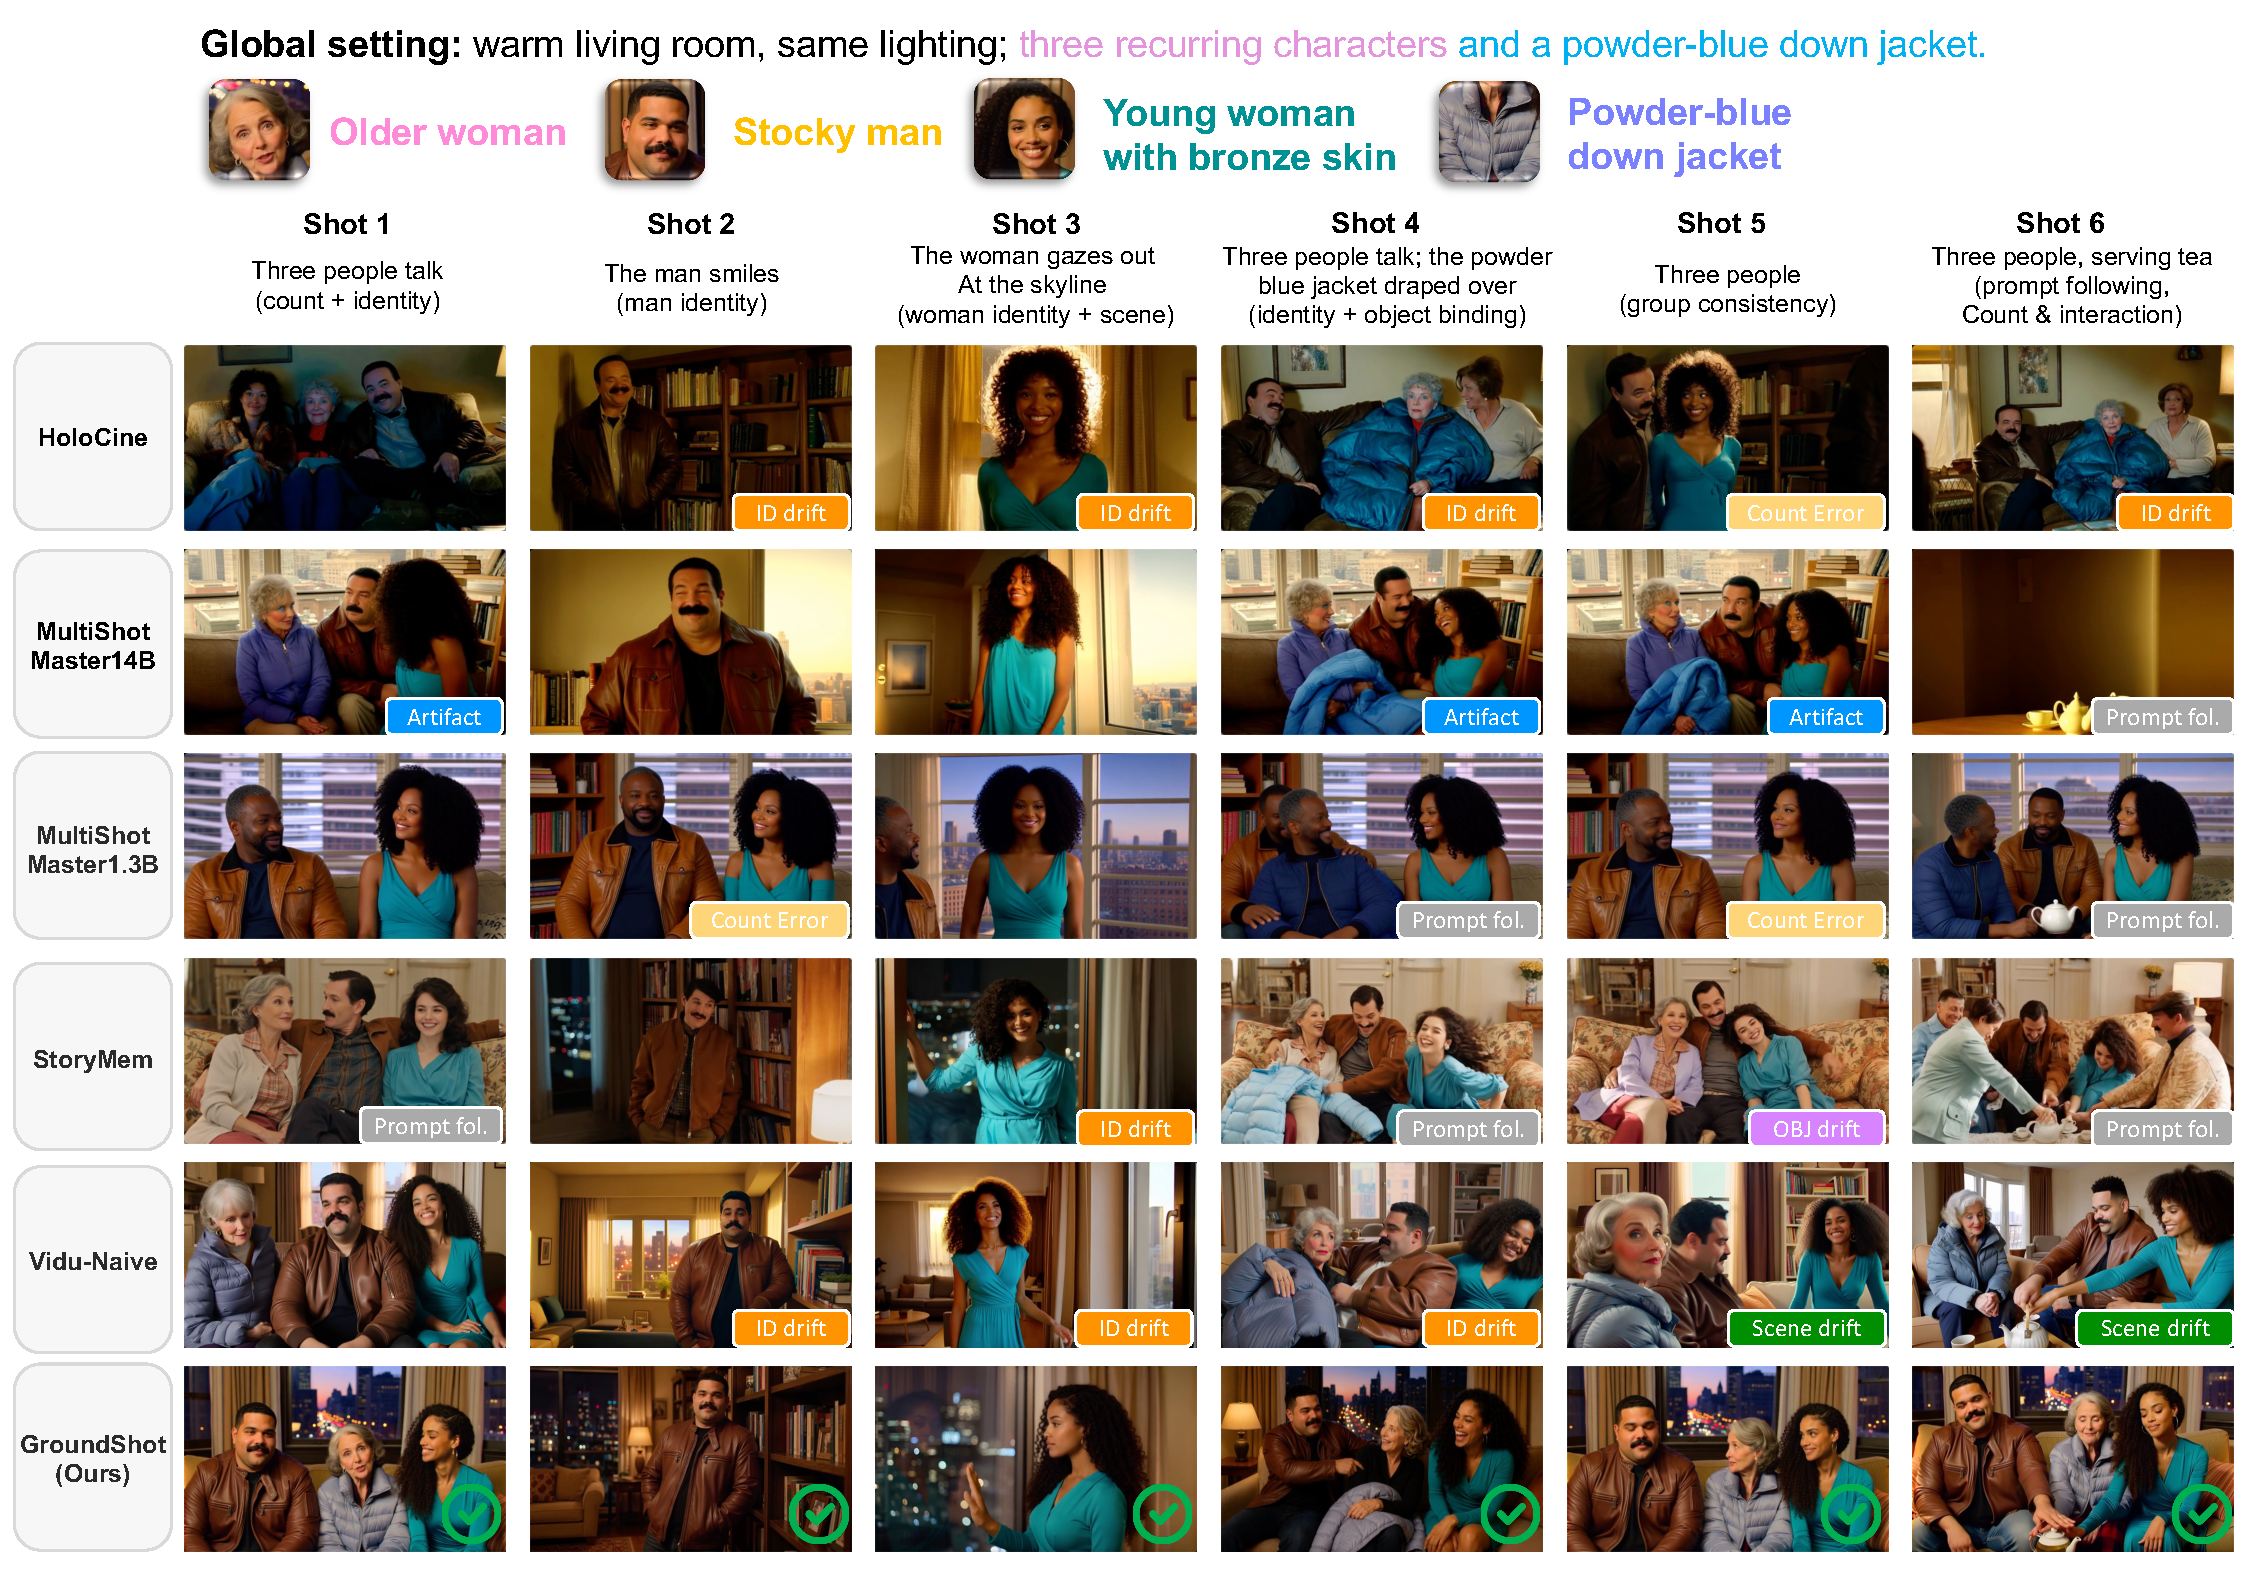
\includegraphics[width=0.95\textwidth]{figures/quality_new.pdf}
    \caption{Qualitative comparison on a six-shot living-room script. The setting contains three recurring characters and a powder-blue down jacket, testing identity/object/scene consistency, character-count correctness, and prompt following. GroundShot preserves the older woman, stocky man, young woman, and jacket across individual and group shots while following the requested actions. Baselines exhibit identity drift, count errors, artifacts, prompt-following failures, object drift, or scene drift.}
    \label{fig:qualitative_comparison}
\end{figure*}

% ============================================================================
\subsection{Ablation Studies}

We ablate the key components of GroundShot to isolate their contributions. All ablations are evaluated on the full GroundBench with identical scripts and seeds.

\begin{table}[t]
\centering
\caption{Ablation study on GroundBench. Each row removes one component from the full system. Entity grounding and scheduling are the two most critical components, together accounting for the majority of GroundShot's gains over baselines.}
\label{tab:ablation}
\vspace{0.3em}
\footnotesize
\setlength{\tabcolsep}{3pt}
\begin{tabular*}{\columnwidth}{@{\extracolsep{\fill}}L{0.36\columnwidth}|ccc|c}
\toprule
\textbf{Configuration} & \textbf{ARC}$\uparrow$ & \textbf{XCD}$\uparrow$ & \textbf{WCI}$\uparrow$ & \textbf{FaceSim}$\uparrow$ \\
\midrule
Full GroundShot              & \textbf{0.426} & \textbf{0.157} & \textbf{0.264} & \textbf{0.449} \\
\midrule
w/o Entity Grounding         & 0.332 & 0.097 & 0.201 & 0.368 \\
w/o Scheduling               & 0.355 & 0.141 & 0.210 & 0.415 \\
w/o Feedback \& Repair       & 0.387 & 0.143 & 0.214 & 0.421 \\
w/o Anchor Protection        & 0.375 & 0.132 & 0.224 & 0.403 \\
w/o Layered Prompt           & 0.401 & 0.136 & 0.238 & 0.432 \\
w/o VLM Selection            & 0.411 & 0.149 & 0.250 & 0.439 \\
\bottomrule
\end{tabular*}
\end{table}

\paragraph{Effect of entity grounding (w/o Entity Grounding).}
Replacing ReferDINO-based entity grounding with naive first-frame extraction removes entity-specific cropping. The system uses the full first frame as a reference, which contains all entities and background---diluting the identity signal for any single entity. This causes the largest overall degradation: ARC drops by $-$0.094, XCD by $-$0.060, and FaceSim by $-$0.081, confirming that entity-level grounding is the most critical component for both anchor quality and multi-character discrimination.

\paragraph{Effect of scheduling (w/o Scheduling).}
Reverting to narrative-order execution forces the system to bootstrap from whatever reference the first appearance provides, even when that appearance is visually poor (e.g., a wide establishing shot). ARC drops by $-$0.071, the second-largest single-component impact, while WCI drops by $-$0.054, indicating that scheduling specifically prevents worst-case anchor failures. The smaller FaceSim drop ($-$0.034) confirms that scheduling primarily benefits anchor-relative evaluation rather than average pairwise similarity.

\paragraph{Effect of remaining components.}
The remaining four components each provide targeted improvements. Removing feedback and repair primarily hurts worst-case robustness (WCI), as occasional catastrophic generations go uncorrected and enter the reference bank. Disabling anchor protection causes progressive drift---each shot conditions on the previous output rather than the stable early-established identity, accumulating errors over longer sequences. Without layered prompting, naive concatenation of global and shot-level text causes entity leakage, where characters from other shots appear prematurely. Finally, replacing VLM-based reference selection with InsightFace scoring removes context-aware pose matching but has the smallest overall impact, suggesting that entity grounding already provides sufficiently discriminative references for most cases.

\paragraph{Effect of visual memory dynamic maintenance.}
The first reliable reference provides the canonical identity standard, but it is not always sufficient for later shots. We explore whether visual memory should stop after this canonical reference, or maintain a compact set of canonical-consistent supplementary references. The canonical reference remains the identity standard throughout: it is protected from replacement and used to gate later memory admission. However, it need not always be the only image passed to the Ref2V model. When a target shot requires a facial expression or camera view that is poorly represented by the canonical reference, a supplementary reference that has already passed the canonical identity gate can provide a better conditioning match.
This distinction is even more important for scenes. Character identity can often be summarized by a strong face or body prototype, but a scene can extend across views as the camera or characters move through the environment. A single scene reference usually shows only a partial static view of a location, while later shots may revisit the same environment from different camera directions or continue into newly visible regions.
Freezing scene memory at the first valid reference can therefore cause several failure modes: the generator may overfit to a partial background crop, lock later shots to an incompatible camera direction or unnaturally jump back to the initial local background even after previous shots have already moved to another part of the same scene.
Visual memory dynamic maintenance admits additional high-quality scene references of the same environment from later reliable shots. Thus, while dynamic maintenance is useful for character expression and view changes, it is often more critical for scenes because scene consistency usually cannot be reduced to one best canonical image.

We therefore qualitatively compare \textbf{Canonical Only}, which freezes entity memory after the first reliable reference, with \textbf{Dynamic Maintenance}, which keeps that canonical anchor while admitting only a few qualified supplementary references. Figure~\ref{fig:dynamic_maintenance_ablation} shows that compact dynamic maintenance remains useful under realistic Ref2V reference limits: these supplementary references provide canonical-consistent coverage for later expressions, views, or scenes, and the scene gains are stronger because multiple references capture complementary regions and camera directions of the same location.

\begin{figure}[t]
    \centering
    \includegraphics[width=0.95\linewidth]{figures/memorygrow.pdf}
    \caption{\textbf{Qualitative effect of visual memory dynamic maintenance.}
    The first two rows show character cases where a single canonical reference preserves identity but does not fully cover later expression and view changes; dynamic maintenance provides identity-safe supplementary references for these target shots. The last two rows show scene cases, where dynamic maintenance is more critical: additional scene references help revisit the same place from a different camera direction and extend the environment along the walking path, instead of forcing later shots to reuse a single local background observation.}
    \label{fig:dynamic_maintenance_ablation}
\end{figure}

% ============================================================================
\subsection{Human Evaluation}

\begin{table}[t]
\centering
\caption{Human evaluation results. Participants rate each method's multi-shot videos on a 1--5 Likert scale across three dimensions. We report mean scores over 40 scripts; higher is better. GroundShot achieves the highest ratings on all dimensions.}
\label{tab:human_eval}
\vspace{0.3em}
\footnotesize
\setlength{\tabcolsep}{3pt}
\begin{tabular*}{\columnwidth}{@{\extracolsep{\fill}}L{0.40\columnwidth}|ccc}
\toprule
\textbf{Method} & \textbf{Identity}$\uparrow$ & \textbf{Text Align.}$\uparrow$ & \textbf{Overall}$\uparrow$ \\
\midrule
HoloCine              & \underline{3.62} & \underline{3.76} & \underline{3.68} \\
MultiShotMaster-1.3B  & 2.78 & 3.55 & 3.18 \\
MultiShotMaster-14B   & 3.21 & 3.70 & 3.34 \\
StoryMem              & 3.48 & 3.72 & 3.60 \\
\midrule
\textbf{GroundShot (Ours)}  & \textbf{4.18} & \textbf{4.23} & \textbf{4.21} \\
\bottomrule
\end{tabular*}
\end{table}

We conduct a questionnaire-based human evaluation with 48 participants on 40 randomly sampled scripts from GroundBench, covering all four diagnostic modules. For each script, participants are shown anonymized multi-shot videos generated by all methods in randomized order. Each participant independently rates every video on a 1--5 Likert scale along three dimensions: \emph{character identity consistency} (whether recurring characters preserve their appearance across shots), \emph{text alignment} (whether each shot matches its description), and \emph{overall quality} (the perceived quality of the complete multi-shot video).

Table~\ref{tab:human_eval} reports the mean scores. GroundShot achieves the highest ratings across all three dimensions, scoring 4.18 on identity consistency. Notably, GroundShot also leads in text alignment (4.23 vs.\ 3.76), indicating that entity-grounded generation does not sacrifice prompt adherence for consistency. The overall quality scores closely track identity ratings, suggesting that human perception of multi-shot video quality is strongly driven by character consistency.

% ============================================================================
\subsection{Discussion}

\begin{figure}[t]
    \centering
    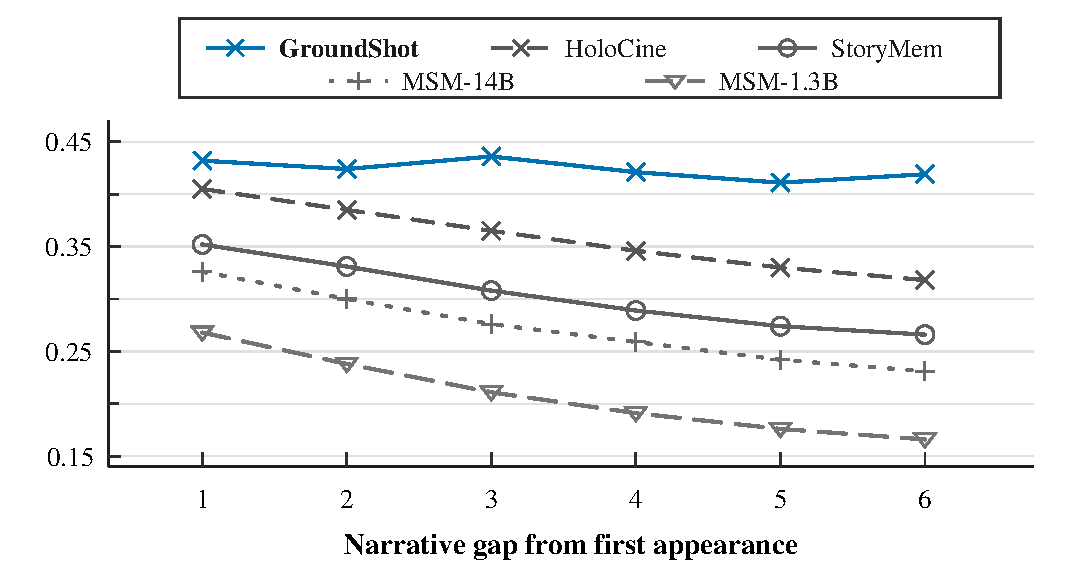
\includegraphics[width=0.98\linewidth]{figures/figure5_arc_curve.pdf}
    \caption{Anchor-relative consistency over narrative distance. The x-axis reports the narrative shot gap from the first valid appearance, and the y-axis reports ARC (higher is better). Baselines tend to decay as the gap increases, whereas GroundShot remains stable with small non-monotonic variation because generation order is decoupled from narrative order and later shots can condition on high-quality canonical references.}
    \label{fig:arc_curve}
\end{figure}

\paragraph{Consistency over narrative distance.}
Figure~\ref{fig:arc_curve} visualizes how ARC changes as recurring entities move farther from their first valid appearance in the final narrative order. For methods that follow narrative order or rely on frame/keyframe memory, ARC tends to decrease with larger gaps, reflecting memory aging and accumulated identity drift. GroundShot shows a different pattern: its ARC stays in a narrow high range rather than forming a monotonic decay. This is expected because the scheduler may generate an informative close-up or medium shot before its narrative neighbors, establish it as a canonical reference, and then condition later narrative positions on that same reference. The remaining variation mainly reflects local shot difficulty, such as occlusion, scale, viewpoint, or interaction, rather than distance along a generation chain.

\paragraph{Reliability of scene references.}
Location memory has a different failure mode from character and object memory. A scene reference cannot be obtained by simply cropping a foreground entity; it must remove foreground subjects and preserve or reconstruct the background. If this reconstruction leaves blocky regions, smeared textures, or residual human figures, reference-conditioned generation may reproduce these artifacts in later shots. GroundShot therefore admits a reconstructed scene only when validation confirms that the unmasked background remains intact, the masked region is plausibly filled, and no prominent foreground subject remains. When this validation fails, especially in close-up shots with little usable background, the system skips the location update rather than storing a weak scene reference. This is usually preferable because such close-up backgrounds carry limited scene identity information, while text prompts can still preserve lighting and setting context until a clearer scene view appears.

\paragraph{Computational overhead and trade-offs.}
GroundShot introduces additional test-time computation because generated shots may be verified by a VLM critic and regenerated when severe failures are detected. This overhead is bounded and measured explicitly. On GroundBench, GroundShot averages 1.20 video generation calls per final shot, with 83.1\% of shots passing on the first attempt; regeneration is therefore occasional rather than the default.
With batched script parsing and risk-gated verification, GroundShot uses 2.3 VLM critique calls and 3.4 text-only LLM calls per script on average, amortized across roughly six shots. Entity-level grounding runs locally with ReferDINO.

To verify that the gains do not simply come from extra generations, we evaluate GroundShot without feedback and repair (Table~\ref{tab:ablation}). This one-generation-per-shot variant still outperforms the strongest external baselines on ARC and FaceSim, showing that scheduling and grounded memory provide the main consistency gains; the full critique-and-retry loop mainly improves worst-case robustness. When latency or budget is the primary constraint, users can disable this loop and retain most of the consistency benefit. GroundShot still inherits the quality ceiling of its video generation backend: if the backend cannot produce a recognizable entity in any single attempt, retries may not resolve the issue.
